%!TEX root = ../main.tex
For the handwriting to be effective we had to bring the data into a clean state. To this end we used a pipeline which is described below in figure \ref{fig:pipeline}. 

\begin{figure}[ht]
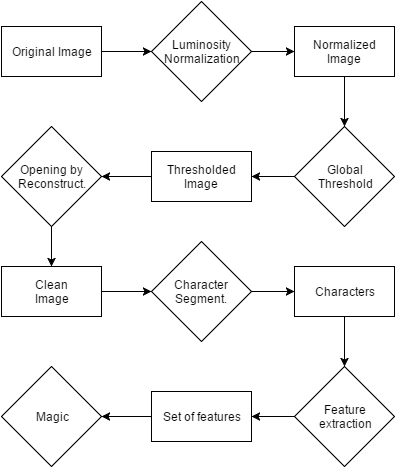
\includegraphics[width=8cm]{shared/img/pipeline.png}
\caption{Overview of our pipeline.}
\label{fig:pipeline}
\end{figure}

As the figure explains the first step is to normalize the luminosity of the image. This step is essential for the thresholding to work since in some parts of dataset the ink has worn off the pages. \Cref{fig:methods:preprocessing:lumNormalization} gives an example why luminosity normalization was necessary. In the above mentioned figure, we applied the same threshold filter with and without luminosity normalization and the results speak for themselves. By normalizing the luminosity we eliminate the need to adjust threshold values in later steps.

\begin{figure}
	\centering
	\subfloat[]{
		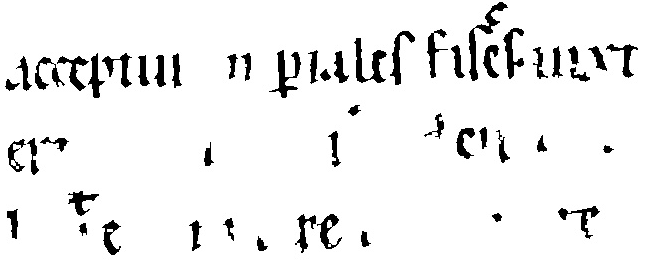
\includegraphics[width=\columnwidth]{shared/img/before_lum.png}%
		\label{fig:methods:preprocessing:lumNormalization:before}%
	}
	\hfil
	\subfloat[]{
		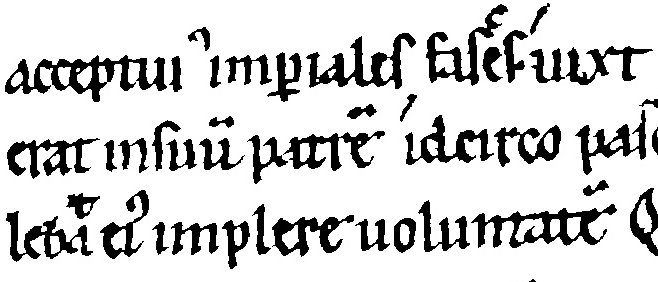
\includegraphics[width=\columnwidth]{shared/img/after_lum.png}%
		\label{fig:methods:preprocessing:lumNormalization:after}%
	}
	\caption{An image of text \protect\subref{fig:methods:preprocessing:lumNormalization:before} before and \protect\subref{fig:methods:preprocessing:lumNormalization:after} after luminization normalization.}
	\label{fig:methods:preprocessing:lumNormalization}
\end{figure}

The next step is to binarize the image and extract the clean text from it. For the binarization we tested the Otsu approach and global threshold and we settled with the first as it gave better results. To eliminate the what is left from the noise we applied opening by reconstruction. This has a result to miss some punctuation characters which however did not prove crucial to our learning process. %In figure \ref{} we can see the final result of the preprocessing of the data. 